\documentclass[a4paper,11pt]{article}

\usepackage[english,greek]{babel}

\newcommand{\lt}{\latintext}
\newcommand{\gt}{\greektext}

\usepackage{amsmath}
\usepackage[pdftex]{graphicx}
\usepackage{verbatim}
\usepackage{parskip}
\usepackage{multirow}

\setlength{\parindent}{15pt}

\title{2η Υποχρεωτική Εργασία \\ Αριθμητική Ανάλυση}
\author{Κωνσταντινίδης Κωνσταντίνος  \\ ΑΕΜ: 4310}
\date{\today}

\begin{document}
\maketitle

\section*{Εισαγωγή}
% ---- ---- ---- ---- ---- ---- ---- ---- ---- ---- ---- ---- ---- ----
% ΕΙΣΑΓΩΓΗ
% ---- ---- ---- ---- ---- ---- ---- ---- ---- ---- ---- ---- ---- ----
    Για την επίλυση όλων των ασκήσεων χρησιμοποιήθηκε η γλώσσα {\textbf{{\lt python}}, με τις 
    βιβλιοθήκες {\textbf{\lt pylab}}  και {\textbf{\lt numpy}}  για την δημιουργία γραφημάτων και τον υπολογισμό μαθηματικών πράξεων. Για κάθε άσκηση, έχουν δημιουργηθεί κλάσεις που υλοποιούν τις 
    μεθόδους, οπότε υπάρχει ένα αντικείμενο για κάθε άσκηση στην {\lt main} και την λύνει.
\section*{Άσκηση 5}
% ---- ---- ---- ---- ---- ---- ---- ---- ---- ---- ---- ---- ---- ----
%ΑΣΚΗΣΗ 5
% ---- ---- ---- ---- ---- ---- ---- ---- ---- ---- ---- ---- ---- ----
Για την εφαρμογή των προσεγγιστικών μεθόδων, πολυωνυμικών, {\lt splines} και ελαχίστων τετραγώνων, για την προσέγγιση τιμών του ημιτόνου στο διάστημα $x\in[-\pi,\pi]$, τα 10 σημεία που χρησιμοποιήθηκαν είναι τα εξής:  
    \begin{center}
    \begin{tabular}{|c|c|}
          \hline
         $x$ & $y=\sin{x}$\\
          \hline
         $-3.1416$ & $0.0$ \\
          \hline
         $-2.60$ & $-0.5155$ \\
          \hline
         $-1.3$ & $-0.9636$ \\
          \hline
         $-0.6$ & $-0.5646$ \\
          \hline
          $0.0$ &  $0.0$ \\ 
          \hline
          $0.5$ &  $0.4794$ \\ 
          \hline
          $0.75$ &  $0.6816$ \\ 
          \hline
          $1.7$ &  $0.9917$ \\ 
          \hline
          $2.75$ &  $0.3817$ \\
          \hline
          $3.1416$ &  $0.0$ \\
          \hline
    \end{tabular}
    \end{center}
Τα παραπάνω αρχικά σημεία είναι μη ομοιόμορφα κατανεμημένα, για μεγαλύτερη ακρίβεια της προσεγγιστικής τιμής. \\
\begin{description}
\item[α)]{\textbf{\lt Lagrange}}\\
Η πολυωνυμική προσέγγιση γίνεται με την εφαρμογή του πολυωνύμου {\lt Lagrange} που δίνεται από την παρακάτω σχέση:
\begin{equation}
    p_n(x) = \sum_{i=0}^{n}y_iL_i(x), i=0,1,...,n  \tag{5.1}\label{eq:lagrange}
\end{equation}
Με $L_i$ οι συντελεστές {\lt Lagrange} με τύπο:
\begin{equation}
    L_i(x) = \frac{(x-x_0)...(x-x_{i-1})(x-x_{i+1})...(x-x_n)}
    {(x_i-x_0)...(x_i-x_{i-1})(x-x_{i+1})...(x_i-x_n)}, i=0,1,...,n    \tag{5.2}\label{eq:lagrange_Li}
\end{equation}

\textbf{Αλγόριθμος:}\\\\
Η συνάρτηση {\lt lagrange} δέχεται ένα σημείο $x\in[-\pi,\pi]$ σαν όρισμα, αρχικοποιούμε την μεταβλητή $n$ με το πλήθος των δοσμένων σημείων και την μεταβλητή $result$ που είναι το αποτέλεσμα του αθροίσματος:
    \lt
    \begin{verbatim}
                def lagrange(self, x):
                    n = len(self.points)
                    result = 0
    \end{verbatim}
    \gt
    Έπειτα εκτελείτε η σχέση \eqref{eq:lagrange}, καλώντας την συνάρτηση $L_i$, εκτελώντας δηλαδή την σχέση \eqref{eq:lagrange_Li} και επιστρέφει το αποτέλεσμα:
    \lt
    \begin{verbatim}
                for i in range(n):
                    result += self.points[i][1]*self.Li(i,x)
                return result
    \end{verbatim}
    \gt
    Η συνάρτηση $L_i$ δέχεται 2 ορίσματα, το $i$ και το $x$, ξεκινάει μία {\lt for loop} που εκτελέι την σχέση \eqref{eq:lagrange_Li}, αγνοώντας την $i$-οστή επανάληψη:
    \lt
    \begin{verbatim}
                def Li(self,i, x):
                    n = len(self.points) # total points
                    result = 1
                    for j in range(n):
                        if j==i:
                            continue
                        result *= (x-self.points[j][0])/\
                        (self.points[i][0]-self.points[j][0])
                    return result
    \end{verbatim}
    \gt
    \newpage
\item[β)]{\textbf{\lt Splines}}\\
Η συνάρτηση του ημιτόνου, στο διάστημα $x\in[-\pi,\pi]$, με $x_0<x_1<…<x_i<...<x_n$ με $i=0,1,...,n$ αποτελεί φυσική καμπύλη {\lt spline}, αφού $\sin''{x} = -\sin{x}$, με $\sin{-\pi} = \sin{\pi} = 0$, που αποτελεί τελική συνθήκη. Αυτό μας οδηγεί από ένα σύστημα $3n-5$ εξισώσεων και $3n-3$ αγνώστων, σε σύστημα $3n-3$ εξισώσεων/αγνώστων. Σκοπός είναι να υπολογίσουμε την $S_i = y_{i} + b_i(x-x_i) + c_i(x-x_i)^2 + d_i(x-x_i)^3$ με $i=0,1,...,n-1$, και να προσεγγίσουμε μία τιμή $x$ με $x_i<x<x_{i+1}$ για κατάλληλο $i$.

Εφαρμόζοντας τις ιδιότητες των φυσικών {\lt splines}, καταλήγω στις σχέσεις για $b_i$ και $d_i$:
    \lt
    \begin{equation}
        d_i = \frac{c_{i+1}-c_i}{3\delta_i} \tag{5.3}\label{eq:di}
    \end{equation}
    \begin{equation}
        b_i = \frac{\Delta_i}{\delta_i} - \frac{\delta_i}{3}(2c_i+c_{i+1}) \tag{5.4}\label{eq:bi}
    \end{equation}
    \gt
Όπου $\Delta_i = y_{i+1} - y_i$ και $\delta_i = x_{i+1} - x_i$ για $i=0,1,...,n-1$.\\
Ενώ συνδυάζοντας τις ιδιότητες και τις παραπάνω σχέσεις, καταλήγω σε ένα σύστημα $n$ αγνώστων $c_i$ της μορφής {\lt Ax = b}:\\
    \begin{equation*}
    \begin{bmatrix}
    1 & 0 & 0\\
    \delta_0 & 2\delta_0+2\delta_1 & \delta_1 & \ddots\\
    &\ddots & \ddots & \ddots & \ddots \\
    & & & & \delta_{n-2} & 2\delta_{n-2}+2\delta_{n-1} & \delta_{n-1} \\
    & & & & 0 & 0 & 1
    \end{bmatrix}
    \begin{bmatrix}
    c_1\\
    \\
    \vdots \\
    \\
    c_n
    \end{bmatrix}
    =     
    \begin{bmatrix}
    0\\
    3(\frac{\Delta_1}{\delta_1}-\frac{\Delta_0}{\delta_0})\\
    \vdots \\
    3(\frac{\Delta_{n-1}}{\delta_{n-1}}-\frac{\Delta_{n-2}}{\delta_{n-2}})\\
    0
    \end{bmatrix}
    \tag{5.5}\label{eq:ci}
    \end{equation*}
    
Λύνοντας το παραπάνω σύστημα, έχουμε όλες τις $S_i$.

\textbf{Αλγόριθμος:}\\\\
Καλούμε την συνάρτηση {\lt splines}, με όρισμα την τιμή του $x$ που θέλουμε να εκτιμήσουμε. Αρχικοποιείτε η μεταβλητή $n$ ως το πλήθος των σημείων, καθώς και οι πίνακες $a$, $dx$, $dy$, με τιμή 0 σε όλες τις θέσεις. Έπειτα υπολογίζουμε τα στοιχεία αυτών των πινάκων. Ο $a$ αντιπροσωπεύει τα $y_i$, ο $dx$ τα $\delta_i$ και ο $dy$ τα $\Delta_i$: 

    \lt
    \begin{verbatim}
            def splines(self, x):
                n = len(self.points)
                a = zeros((n,1))
                dx = zeros((n-1,1))
                dy = zeros((n-1,1))

                for i in range(n-1):
                    a[i] = self.points[i][1]
                    dx[i] = self.points[i+1][0] - self.points[i][0]        
                    dy[i] = self.points[i+1][1] - self.points[i][1]   
    \end{verbatim}
    \gt

Δημιουργείτε ο πίνακας $A$ που αντιπροσωπεύει τον αριστερό πίνακα στην σχέση \eqref{eq:ci}, και ο πίνακας $r$, ο πίνακας στο δεξιό μέρος της σχέσης \eqref{eq:ci}. Έπειτα υπολογίζονται τα στοιχεία των πινάκων:

    \lt
    \begin{verbatim}
            A = zeros((n,n))
            A[0][0] = 1
            A[n-1][n-1] = 1
            r = zeros((n,1))

            for i in range(1,n-1):
                A[i][i-1] = dx[i-1]
                A[i][i] = 2*(dx[i-1] + dx[i])
                A[i][i+1] = dx[i]
                r[i] = 3*(dy[i]/dx[i] - dy[i-1]/dx[i-1])
    \end{verbatim}
    \gt
Η σχέση \eqref{eq:ci} είναι της μορφής {\lt Ax = b}, οπότε μπορεί να λυθεί με την μέθοδο {\lt PA = LU}. Μετά την λύση του συστήματος, υπολογίζονται τα $b_i$ και $d_i$. Για την λύση του συστήματος χρησιμοποιείτε η συνάρτηση {\lt Gauss}:

    \lt
    \begin{verbatim}
            c = Gauss(A,r) # Solve for ci

            b = zeros((n-1,1))
            d = zeros((n-1,1))
            for i in range(n-1):
                d[i] = (c[i+1]-c[i])/(3*dx[i]) 
                b[i] = dy[i]/dx[i] - (dx[i]/3)*(2*c[i]+c[i+1])
    \end{verbatim}
    \gt

    
Τέλος, βρίσκουμε την κατάλληλη $S_i$ ώστε $x_i<x<x_{i+1}$ και επιστρέφουμε την τιμή της $S_i(x)$: 

    \lt
    \begin{verbatim}
        for i in range(n-1):
            if self.points[i][0]<x<self.points[i+1][0]:
                return a[i]+b[i]*(x-self.points[i][0]) + \
                       c[i]*(x-self.points[i][0])**2 + \
                       d[i]*(x-self.points[i][0])**3
    \end{verbatim}
    \gt
\item[γ)]{\textbf{ Μέθοδος Ελαχίστων Τετραγώνων}}\\
Στην μέθοδο ελαχίστων τετραγώνων, αναζητούμε μία καμπύλη $n$-τάξης, που ταιριάζει καλύτερα στα δοθέντα σημεία. Για αυτή την άσκηση, χρησιμοποιείτε καμπύλη 3ης τάξης, δηλαδή η καμπύλη θα είναι της μορφής $y = c_0 + c_1t + c_2t^2+c_3t^3$, οπότε και αναζητούμε τα $c$. Αφού τα σημεία ουσιαστικά είναι πάνω στην καμπύλη, επαληθεύουν την εξίσωσή της. Άρα κάνοντας αντικατάσταση τα σημεία στην εξίσωση, έχουμε όσες εξισώσεις με αγνώστους $c$, όσα και τα σημεία. Αυτό το σύστημα όμως αδύνατο, οπότε χρησιμοποιούμε το σύστημα $A^TAx' = A^Tb$, και έτσι βρίσκουμε τους συντελεστές $c$, οπότε και την συνάρτηση $y$.\\

    \textbf{Αλγόριθμος:}\\\\
Καλούμε την συνάρτηση {\lt leastSquares3} με ορίσματα μία λίστα με τα δεδομένα σημεία, και το $x$ που θα εκτιμηθεί. Αρχικοποιείτε η μεταβλητή $n$ ως το πλήθος των σημείων, και με μία επανάληψη, δημιουργούνται οι πίνακες $A$ και $b$. Αφού θέλουμε 3η τάξη, ο $A$ θα έχει 4 στήλες, όσοι και οι άγνωστοι συντελεστές:

    \lt
    \begin{verbatim}
        def leastSquares3(x, points):
            n = len(points)
            A = zeros((n,4))
            b = zeros((n,1)) 
            for i in range(n):
                A[i][0] = 1
                A[i][1] = points[i][0]
                A[i][2] = points[i][0]**2
                A[i][3] = points[i][0]**3
                b[i] = points[i][1]
    \end{verbatim}
    \gt
    
Υπολογίζονται οι πίνακες $A^TA$ και $A^Tb$, λύνεται το σύστημα $A^TAx' = A^Tb$ με την συνάρτηση {\lt Gauss}, και επιστρέφεται η τιμή $y(x)$:

    \lt
    \begin{verbatim}
            ATA = dot(transpose(A),A)
            ATb = dot(transpose(A),b)
            c = Gauss(ATA,ATb)
            return c[0] + x * c[1] + c[2]*x**2 + c[3]*x**3
    \end{verbatim}
    \gt

\end{description}

\textbf{Αποτελέσματα:}\\
Αποτελέσματα προσεγγίσεων της τιμής $x=\pi/12$:
    \lt
    \begin{verbatim}
                            Approximation of pi/12

                    Actual: 0.25882

                    Lagrange: 0.25882
                    Error: 0.0000001

                    Splines: 0.25857
                    Error: 0.0002486

                    LeastSquares(3): 0.22625
                    Error: 0.0325700
    \end{verbatim}
    \gt
Παρατηρούμε για τον υπολογισμό της $sin(\pi/12)$ ότι με την μέθοδο {\lt Lagrange} έχουμε 6 ψηφία ακρίβειας, με την μέθοδο των {\lt splines} 2 και για την μέθοδο ελαχίστων τετραγώνων, 1.

Τα σφάλματα των αποτελεσμάτων των υπολογισμών 200 τυχαίων σημείων:
\begin{center}
    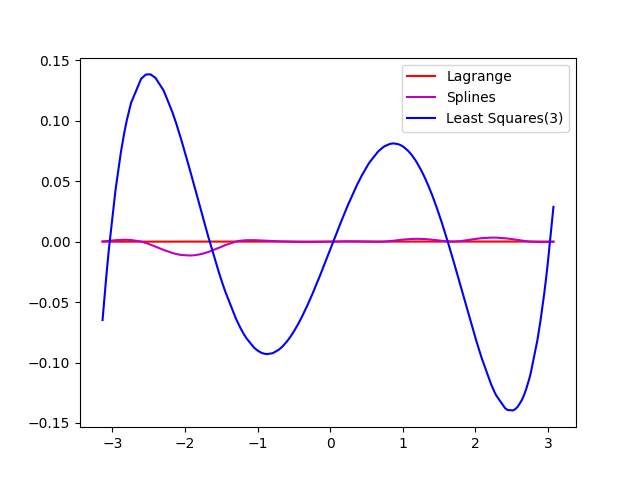
\includegraphics[scale=0.65]{sfalmata.png}
\end{center}
    \lt
    \begin{verbatim}
        Max Lagrange error:  5.76474715763553e-05
        Max splines error:  0.01151239
        Max least squares error:  0.13958598
    \end{verbatim}
    \gt
Άρα για 10 δεδομένα σημεία, πετυχαίνουμε ακρίβεια 4 δεκαδικών με την μέθοδο {\lt Lagrange}, 1 δεκαδικό με την μέθοδο των {\lt splines} και ακρίβεια 0 δεκαδικών με την μέθοδο ελαχίστων τετραγώνων.
\newpage
\section*{Άσκηση 6}
% ---- ---- ---- ---- ---- ---- ---- ---- ---- ---- ---- ---- ---- ----
%ΑΣΚΗΣΗ 6
% ---- ---- ---- ---- ---- ---- ---- ---- ---- ---- ---- ---- ---- ----
\begin{description}
\item[α)]{\textbf{ Μέθοδος τραπεζίου}}\\
Ο τύπος της μεθόδου τραπεζίου για την προσέγγιση της τιμής του ολοκληρώματος της $f(x)$ για $x\in[a,b]$, είναι:
\begin{equation}
    \int_{a}^{b}f(x)dx \cong \frac{b-a}{2N}(f(x_0)+f(x_N) + 2\sum_{i=1}^{N-1}f(x_i)) \tag{6.1}\label{eq:trapezoid}
\end{equation}
Με σφάλμα: 
\begin{equation}
    |e| \leq \frac{(b-a)^3}{12N^2}M  \tag{6.2}\label{eq:trapezoiderror}
\end{equation}
Όπου $M$, μέγιστη απόλυτη τιμή της $f''$ για  $x\in[a,b]$.\\\\
\textbf{Αλγόριθμος:}\\\\
Καλούμε την συνάρτηση {\lt trapezoidRule}. Πρώτο βήμα είναι ο υπολογισμός των $f(x)$. Αυτό γίνεται από την συνάρτηση {\lt calculateFx}, που δημιουργεί μία λίστα $x$, που περιέχει τα $x_i$, με $x_i = a + \frac{i(b-a)}{n})$, δηλαδή χωρίζει το διάστημα σε μικρότερα διαστήματα ίσης απόστασης. Έπειτα υπολογίζει και επιστρέφει τα $f(x)$, που για την άσκηση έχουμε $f(x) = \sin(x)$:

    \lt
    \begin{verbatim}
    def TrapezoidRule(self):
        y = self.calculateFx()
        ...
    def calculateFx(self):
        # n is number of parabols and NOT amount of points
        x = [self.a+i*(self.b-self.a)/self.n for i in range(self.n+1)] 
        y = [self.f(xi) for xi in x]
        return y
        ...
    def f(self,x): return sin(x)
    \end{verbatim}
    \gt
Δημιουργείτε η μεταβλητή {\lt sum}, που είναι ουσιαστικά το αποτέλεσμα της παρένθεσης της σχέσης \eqref{eq:trapezoid}, έπειτα πολλαπλασιάζεται η {\lt sum} με $\frac{b-a}{2N}$, και αποθηκεύεται το αποτέλεσμα την μεταβλητή {\lt In}, που είναι και η προσέγγιση: 

    \lt
    \begin{verbatim}
        sum = y[0] + y[self.n]
        for i in range(1,self.n):
            sum += 2*y[i]
        In = ((self.b-self.a)/(2*self.n))*sum
    \end{verbatim}
    \gt

Υπολογίζεται το σφάλμα, σύμφωνα με τη σχέση \eqref{eq:trapezoiderror}, με $M=\sin(\pi/2)$, που είναι η μέγιστη τιμή της $f(x)$:  

    \lt
    \begin{verbatim}
        M = sin(pi/2)
        e = (((self.b-self.a)**3)*M)/(12*(self.n**2))
    \end{verbatim}
    \gt
    
Τέλος, επιστροφή της προσέγγισης: 

    \lt
    \begin{verbatim}
        return In
    \end{verbatim}
    \gt

\item[β)]{\textbf{Μέθοδος {\lt Simpson}}}\\
Ο τύπος της μεθόδου {\lt Simpson} για την προσέγγιση της τιμής του ολοκληρώματος της $f(x)$ για $x\in[a,b]$, είναι:

\begin{equation}
    \int_{a}^{b}f(x)dx \cong \frac{b-a}{3N}(f(x_0)+f(x_N) + 2\sum_{i=1}^{\frac{N}{2}-1}f(x_{2i}) + 4\sum_{i=1}^{\frac{N}{2}}f(x_{2i-1})) \tag{6.3}\label{eq:simpson}
\end{equation}
Με σφάλμα: 
\begin{equation}
    |e| \leq \frac{(b-a)^5}{180N^4}M  \tag{6.4}\label{eq:simpsonerror}
\end{equation}
Όπου $M$, μέγιστη απόλυτη τιμή της $f^{(4)}$ για  $x\in[a,b]$.\\\\

\textbf{Αλγόριθμος:}\\\\
Καλούμε την συνάρτηση {\lt simpson}. Όπως και παραπάνω, καλείται η {\lt calculateFx}, και μετά υπολογίζεται η σχέση \eqref{eq:simpson}, και αποθηκεύεται το αποτέλεσμα στην μεταβλητή {\lt In}:

    \lt
    \begin{verbatim}
    def simpson(self):
        y = self.calculateFx()
        sum = y[0] + y[self.n]
        for i in range(1, self.n):
            if i%2==0:
                sum += 2*y[i]
            else:
                sum += 4*y[i]
        In = ((self.b-self.a)/(3*self.n))*sum
    \end{verbatim}
    \gt
\newpage
Υπολογίζεται το σφάλμα με την σχέση \eqref{eq:simpsonerror}, και επιστρέφεται η προσέγγιση:

    \lt
    \begin{verbatim}
        # f''''(x) = sinx
        # |Max(f), xE(0/pi/2| = f(pi/2)
        M = sin(pi/2)
        e = (((self.b-self.a)**5)*M)/(180*(self.n**4))

        return In
    \end{verbatim}
    \gt
    
\end{description}

\textbf{Αποτελέσματα:}\\\\
Αποτελέσματα προσέγγισης $\int_{0}^{\pi/2}\sin{x}dx$:
    \lt
    \begin{verbatim}
                Trapezoid rule: 

            Actual value: 1.
            Approximated value: 0.997943
            Theoretical error: 0.003230
            Numeric error: 0.002057

                Simpson's rule:

            Actual value: 1.
            Approximated value: 1.000003
            Theoretical error: 0.000005
            Numeric error: 0.000003

    \end{verbatim}
    \gt
Όπως ήταν αναμενόμενο, η μέθοδος {\lt Simpson} είναι πιο ακριβής.

\section*{Άσκηση 7}
% ---- ---- ---- ---- ---- ---- ---- ---- ---- ---- ---- ---- ---- ----
%ΑΣΚΗΣΗ 7
% ---- ---- ---- ---- ---- ---- ---- ---- ---- ---- ---- ---- ---- ----
Θα εκτιμηθούν οι τιμές κλεισίματος των κλαδικών δεικτών τεχνολογίας (ΔΤΧ) και ενέργειας (ΔΠΑ), έχοντας δεδομένα σημεία, τα κλεισίματα των εξής ημερομηνιών:
\begin{center}
    \begin{tabular}{|c|c|c|c|}
         \hline
         $x_i$& Ημ/νία & ΔΤΧ & ΔΠΑ \\
         \hline
         -6 & 19/4/22 & 2315.99 & 3823.09 \\
         \hline
         -5 &20/4/22 & 2319.55 & 3870.41 \\
         \hline
         -4 &21/4/22 & 2329.25 & 3830.82 \\
         \hline
         1 &26/4/22 & 2299.51 & 3864.31 \\
         \hline
         2 &27/4/22 & 2221.23 & 3822.67 \\
         \hline
         3 &28/4/22 & 2256.81 & 3871.8 \\
         \hline
         4 &29/4/22 & 2249.2 & 3854.22 \\
         \hline
         8 &3/5/22 & 2153.66 & 3751.24 \\
         \hline
         9 &4/5/22 & 2152.46 & 3790.35 \\
         \hline
         10 &5/5/22 & 2065.76 & 3851.0601 \\
         \hline
    \end{tabular}
\end{center}
 Τα $x_i$ είναι τα $x$ των σημείων, που μετρώντας από το 10ο κλείσιμο την ημέρα γενεθλίων (5/5), το πρώτο κλείσιμο έγινε 16 μέρες πριν, οπότε πρέπει να υπολογίσουμε και τις αποστάσεις των κλεισιμάτων, για σωστότερες προβλέψεις. Οι εκτιμήσεις θα γίνουν με την μέθοδο ελαχίστων τετραγώνων 2ου, 3ου και 4ου βαθμού. 
 Οι ημερομηνίες κλεισιμάτων που θα εκτιμηθούν είναι 6/5 και 12/5, άρα τα $x_i$ είναι 11 και 17 αντιστοίχως.\\\\
 
\textbf{Αλγόριθμος:}\\\\
Καλούμε την συνάρτηση {\lt predictions}, αρχικοποιείται ο πίνακας $x$ που περιέχει τα $x_i$, και υπολογίζονται οι συντελεστές με την κλήση της {\lt calculateCoeffs} που επιστρέφει λίστες από τους συντελεστές, για κάθε δείκτη, για κάθε βαθμό ελαχίστων τετραγώνων. Ο υπολογισμός των συντελεστών γίνεται απο κλίσεις των αντιστοίχων συναρτήσεων:

    \lt
    \begin{verbatim}
    def predictions(self):
        x = [point[0] for point in self.pointsDPA]

        c2DTX, c3DTX, c4DTX, c2DPA, c3DPA, c4DPA = self.calculateCoeffs() 
            .....
            
    def calculateCoeffs(self):
        return leastSquares2(self.pointsDTX),\
               leastSquares3(self.pointsDTX),\
               leastSquares4(self.pointsDTX),\
               leastSquares2(self.pointsDPA),\
               leastSquares3(self.pointsDPA),\
               leastSquares4(self.pointsDPA)
    \end{verbatim}
    \gt
    \newpage
Η διαφορά των συναρτήσεων απο την {\lt leastSquares3} που αναλύθηκε παραπάνω, είναι στο μέγεθος πίνακα $A$:

    \lt
    \begin{verbatim}
    
        def leastSquares2(points):
                ....
            for i in range(n):
                A[i][0] = 1
                A[i][1] = points[i][0]
                A[i][2] = points[i][0]**2
                b[i] = points[i][1]
                ....
            
        def leastSquares3(points):
                ....
            for i in range(n):
                A[i][0] = 1
                A[i][1] = points[i][0]
                A[i][2] = points[i][0]**2
                A[i][3] = points[i][0]**3
                b[i] = points[i][1]
                ....
    
        def leastSquares4(points):
                ....
            for i in range(n):
                A[i][0] = 1
                A[i][1] = points[i][0]
                A[i][2] = points[i][0]**2
                A[i][3] = points[i][0]**3
                A[i][4] = points[i][0]**4
                b[i] = points[i][1]
                ....
    \end{verbatim}
    \gt
Αφού υπολογιστούν οι συντελεστές, καλείτε η {\lt solvePolynom} που δέχεται τους συντελεστές και τα $x_i$, και επιστρέφει το αποτέλεσμα, που είναι και η εκτίμηση: 
 
    \lt
    \begin{verbatim}
    def solvePolynom(self, c, x):
        for i in range(5-len(c)):
            c = list(c)
            c.append(0) # if degree < 4 -> add 0 to c list untill size(c) = 4
        return c[0] + x*c[1] + c[2]*x**2+\
               c[3]*x**3 + c[4]*x**4

    \end{verbatim}
    \gt
Η {\lt solvePolynom} υπολογίζει πολυώνυμο 4ου βαθμού, αν οι συντελεστές είναι λιγότεροι, δηλαδή γίνεται υπολογισμός ελαχίστων τετραγώνων 2ου και 3ου βαθμού,προστίθενται μηδενικοί συντελεστές.\\\\
\textbf{Αποτελέσματα:}\\
\begin{center}
    \begin{tabular}{|c|c|c|c|c|c|c|c|c|}
    \hline
    \multicolumn{9}{|c|}{ΔΤΧ}\\\hline
    \multirow{2}{*}{$x_i$} & \multirow{2}{*}{Ημ/νία} & \multirow{2}{*}{\lt Actual} & \multicolumn{2}{|c|}{2ου βαθμού} & \multicolumn{2}{|c|}{3ου βαθμού} & \multicolumn{2}{|c|}{4ου βαθμού}\\\cline{4-9}
    & & & {\lt Pred.} & {\lt Error} & {\lt Pred.} & {\lt Error} & {\lt Pred.} & {\lt Error}\\\hline
    11 & 6/5  & 2017.81  & 2063.436 & -45.626 & 2048.676 & -30.866 & 1995.513 & 22.296   \\\hline
    17 & 12/5 & 1958.42  & 1840.629 & 117.79  & 1694.081 & 264.338 &  694.777 & 1263.642 \\\hline
    \end{tabular}
\end{center}

\begin{center}
    \begin{tabular}{|c|c|c|c|c|c|c|c|c|}
    \hline
    \multicolumn{9}{|c|}{ΔΠΑ}\\\hline
    \multirow{2}{*}{$x_i$} & \multirow{2}{*}{Ημ/νία} & \multirow{2}{*}{\lt Actual} & \multicolumn{2}{|c|}{2ου βαθμού} & \multicolumn{2}{|c|}{3ου βαθμού} & \multicolumn{2}{|c|}{4ου βαθμού}\\\cline{4-9}
    & & & {\lt Pred.} & {\lt Error} & {\lt Pred.} & {\lt Error} & {\lt Pred.} & {\lt Error}\\\hline
    11 & 6/5  & 3813.55  & 3788.412 &  25.137 & 3840.36  &  -26.815 & 3927.134  & -113.584 \\\hline
    17 & 12/5 & 3916.22  & 3710.892 & 205.327 & 4226.651 & -310.431 & 5857.738 & -1941.518 \\\hline
    \end{tabular}
\end{center}
Παρατηρούμε ότι έχουμε μεγάλες αποκλίσεις απο τις πραγματικές τιμές των κλεισιμάτων, ειδικά όσο απομακρυνόμαστε απο την τελευταία δεδομένη ημερομηνία, οπότε κατανοούμε οτι έχοντας δεδομένα μόνο 5 αρχικές τιμές, δεν μπορούμε να κάνουμε αξιόπιστες προβλέψεις.

\end{document}